\setcounter{page}{1}

\section{Introducción}
    Ejemplo de cita~(\cite{buffett84}).
\section{Objetivos}
    \begin{itemize}
        \item Emplear PAT en la interacción de redes privadas - redes públicas.
    \end{itemize}

\section{Desarrollo del Trabajo}

    \begin{figure}[H]
        \centering
        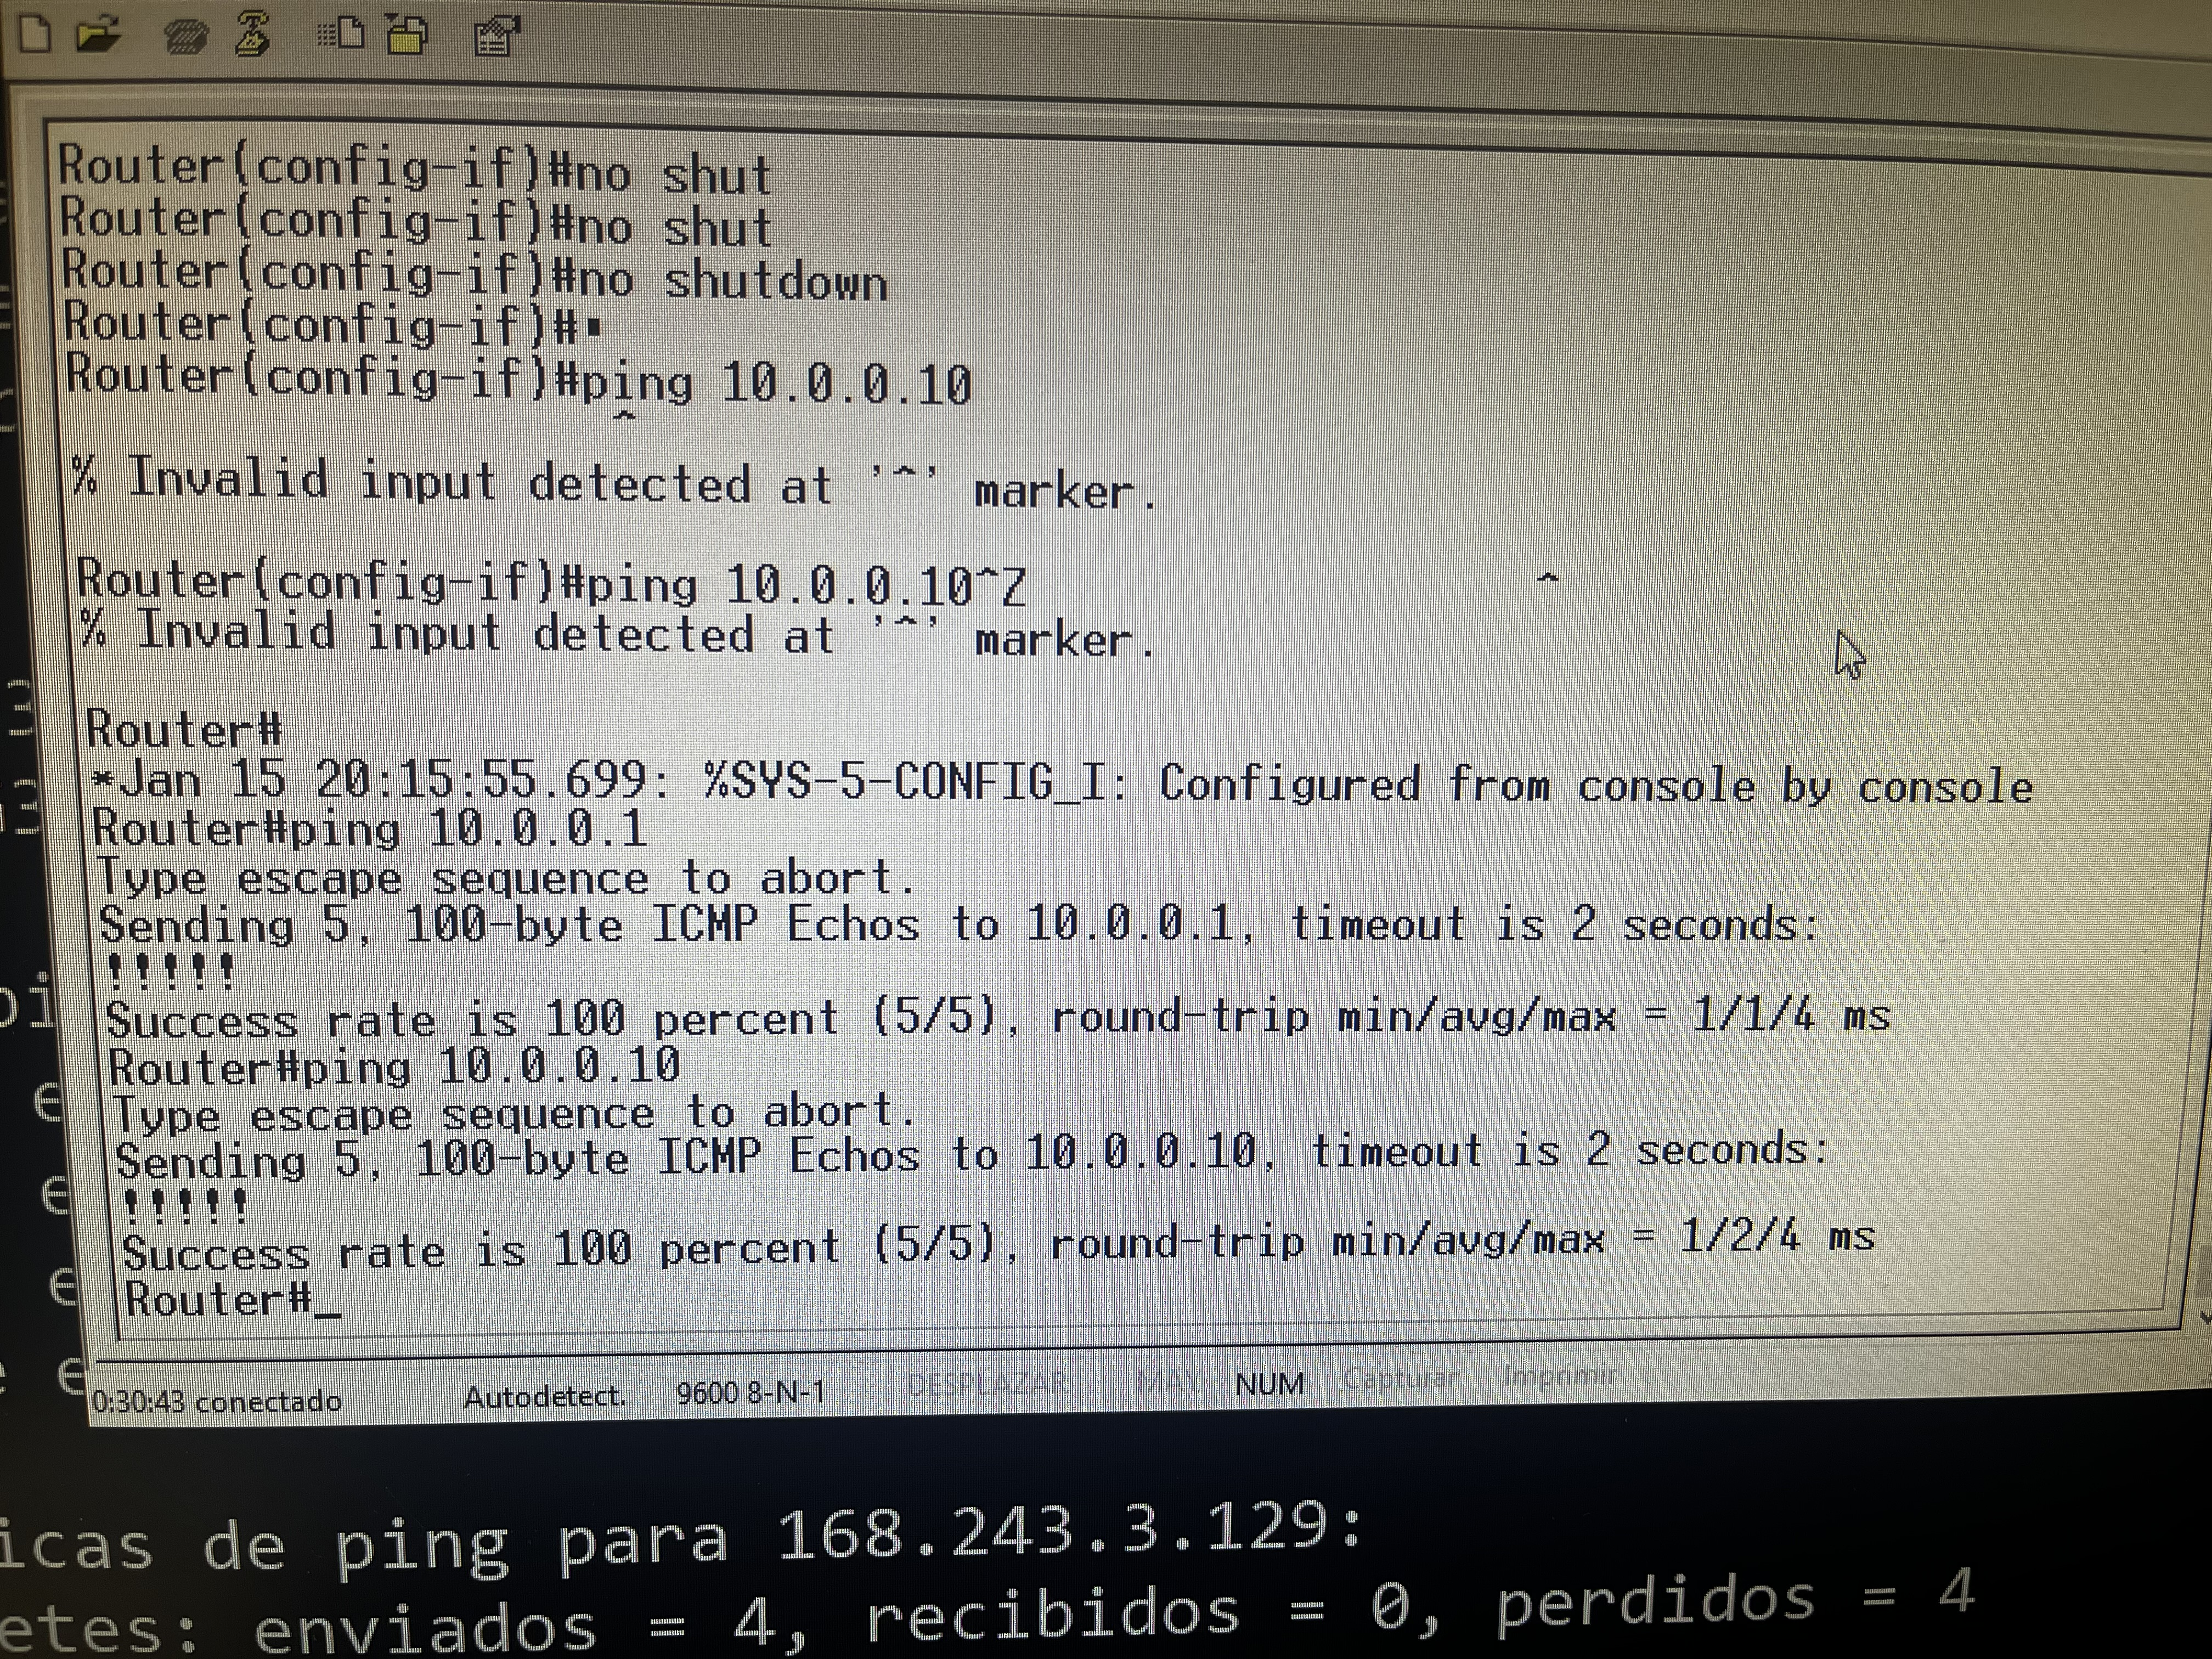
\includegraphics[width=0.8\textwidth]{img/1.jpg}
        \caption{Imagen de Ejemplo}
        \label{fig:Imagen_Ejemplo1}
    \end{figure}

    \begin{figure}[H]
        \centering
        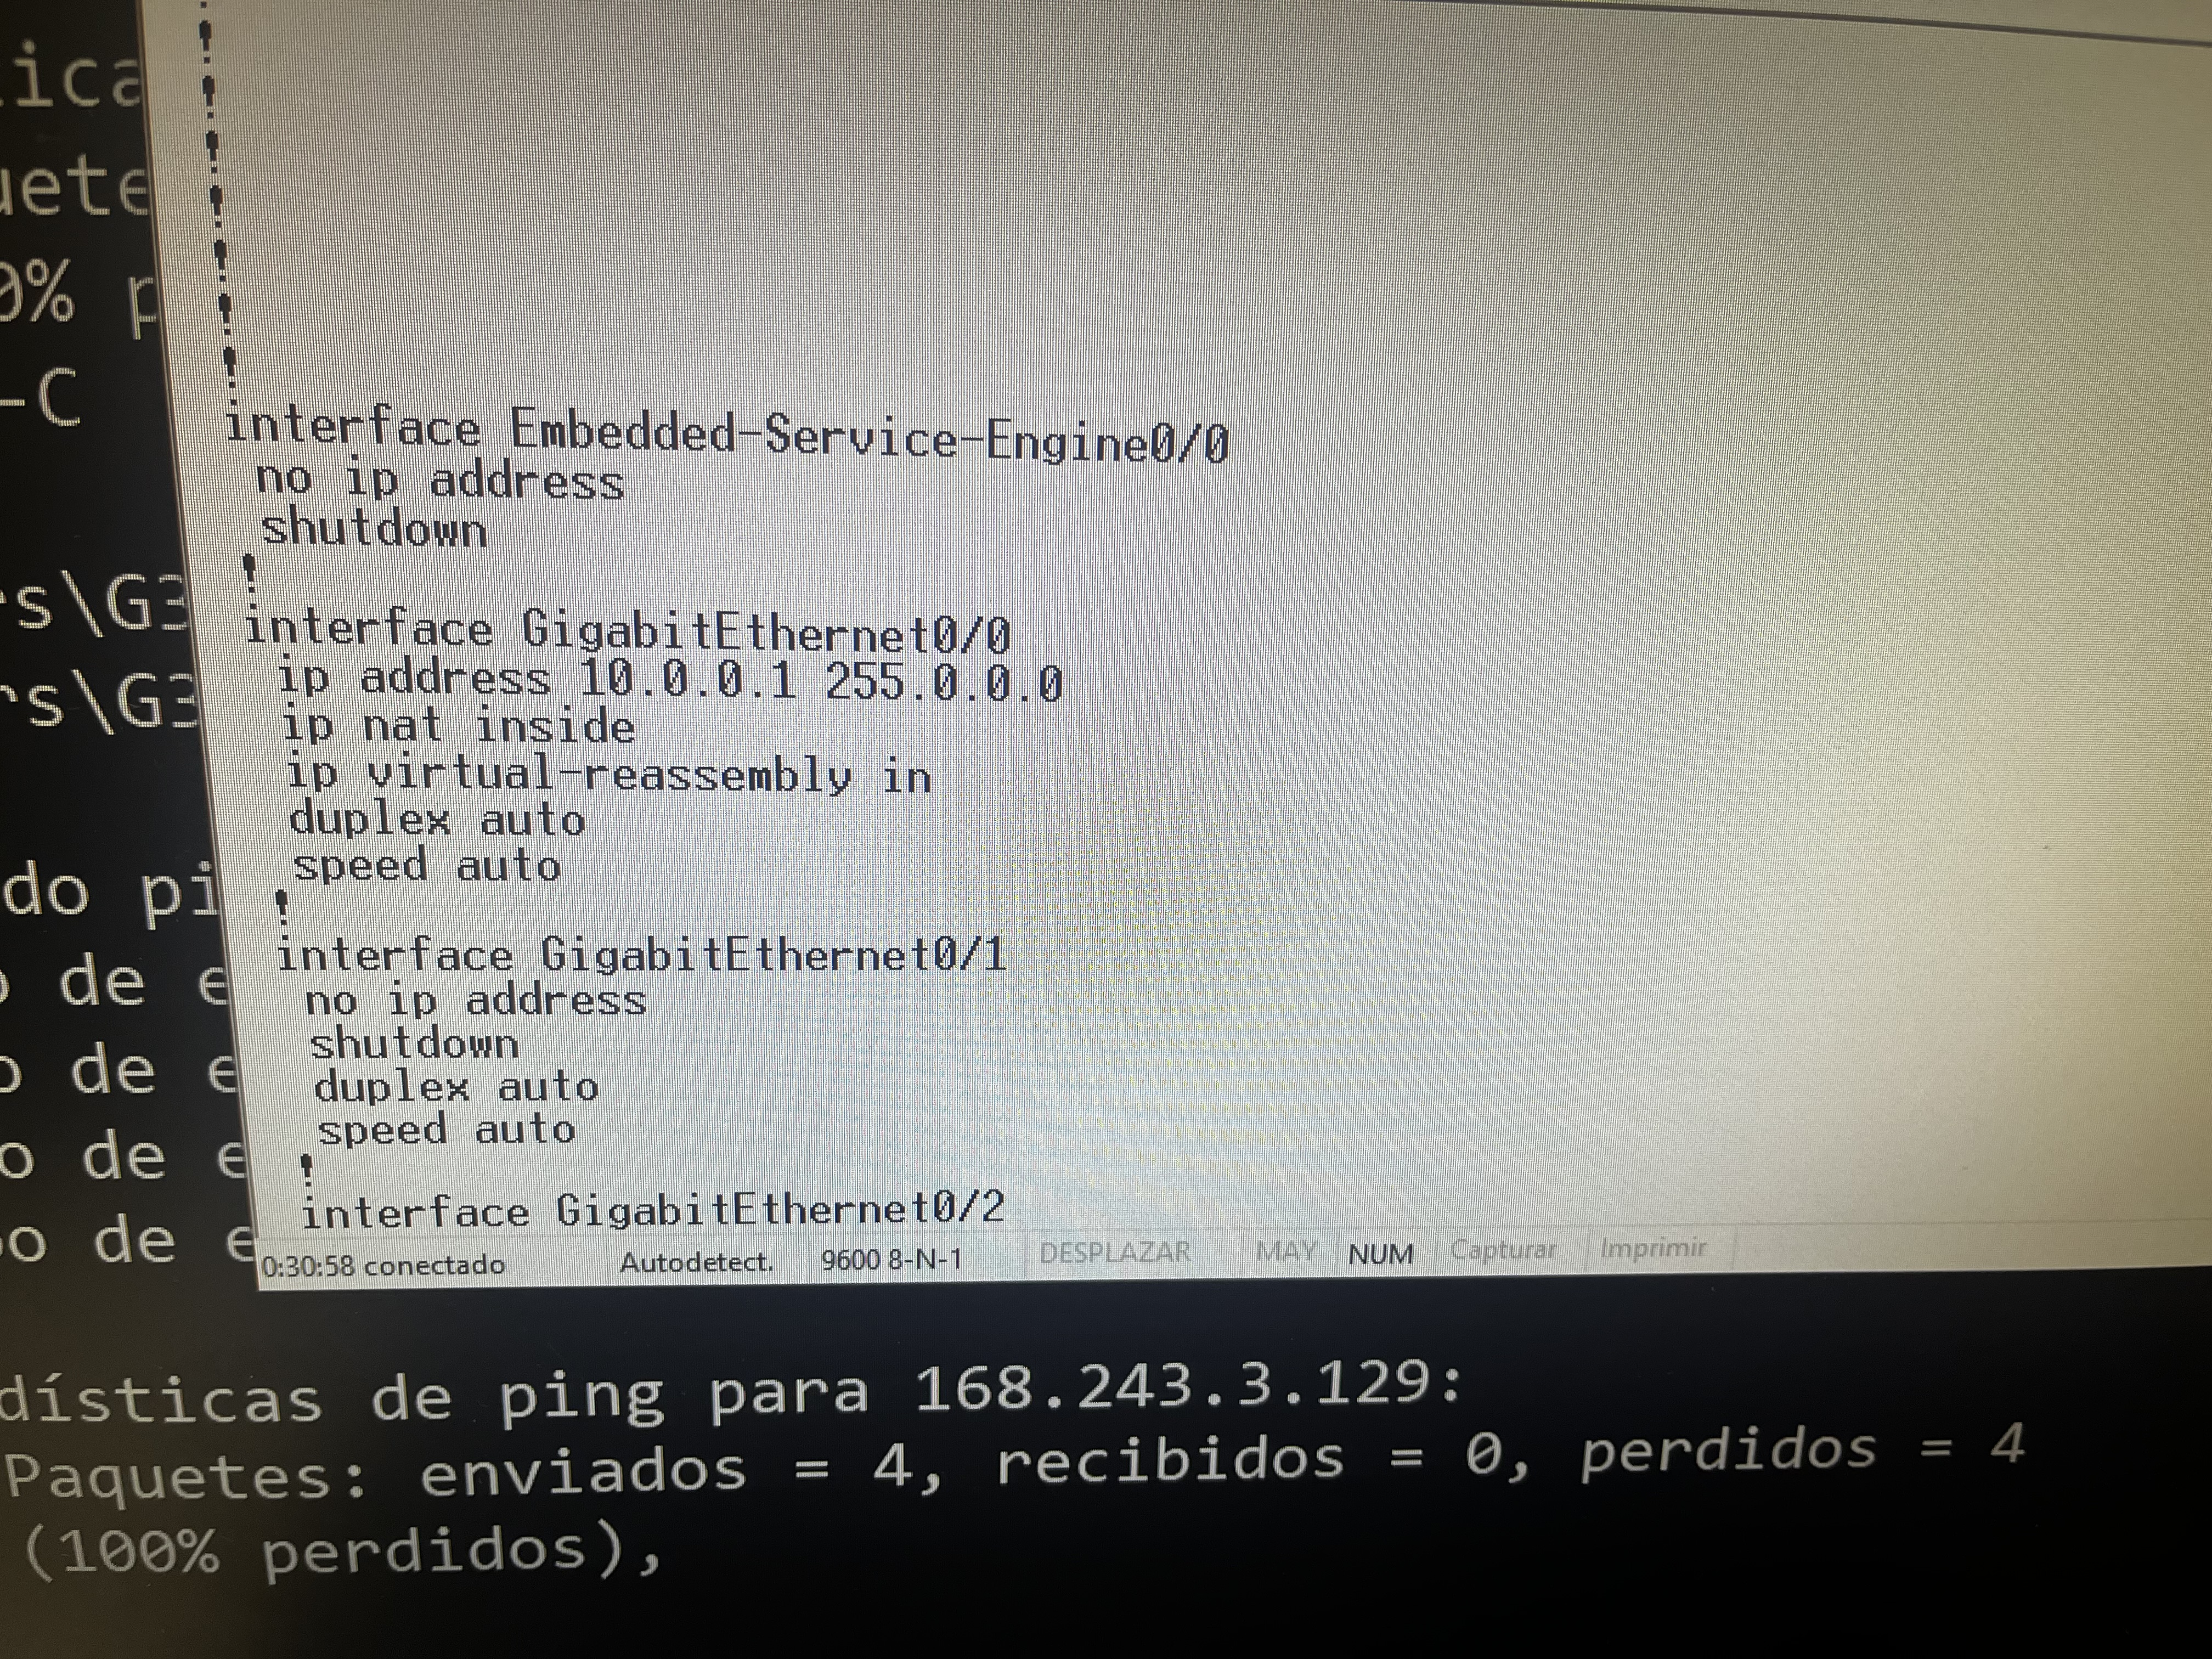
\includegraphics[width=0.8\textwidth]{img/2.jpg}
        \caption{Imagen de Ejemplo}
        \label{fig:Imagen_Ejemplo2}
    \end{figure}

    \begin{figure}[H]
        \centering
        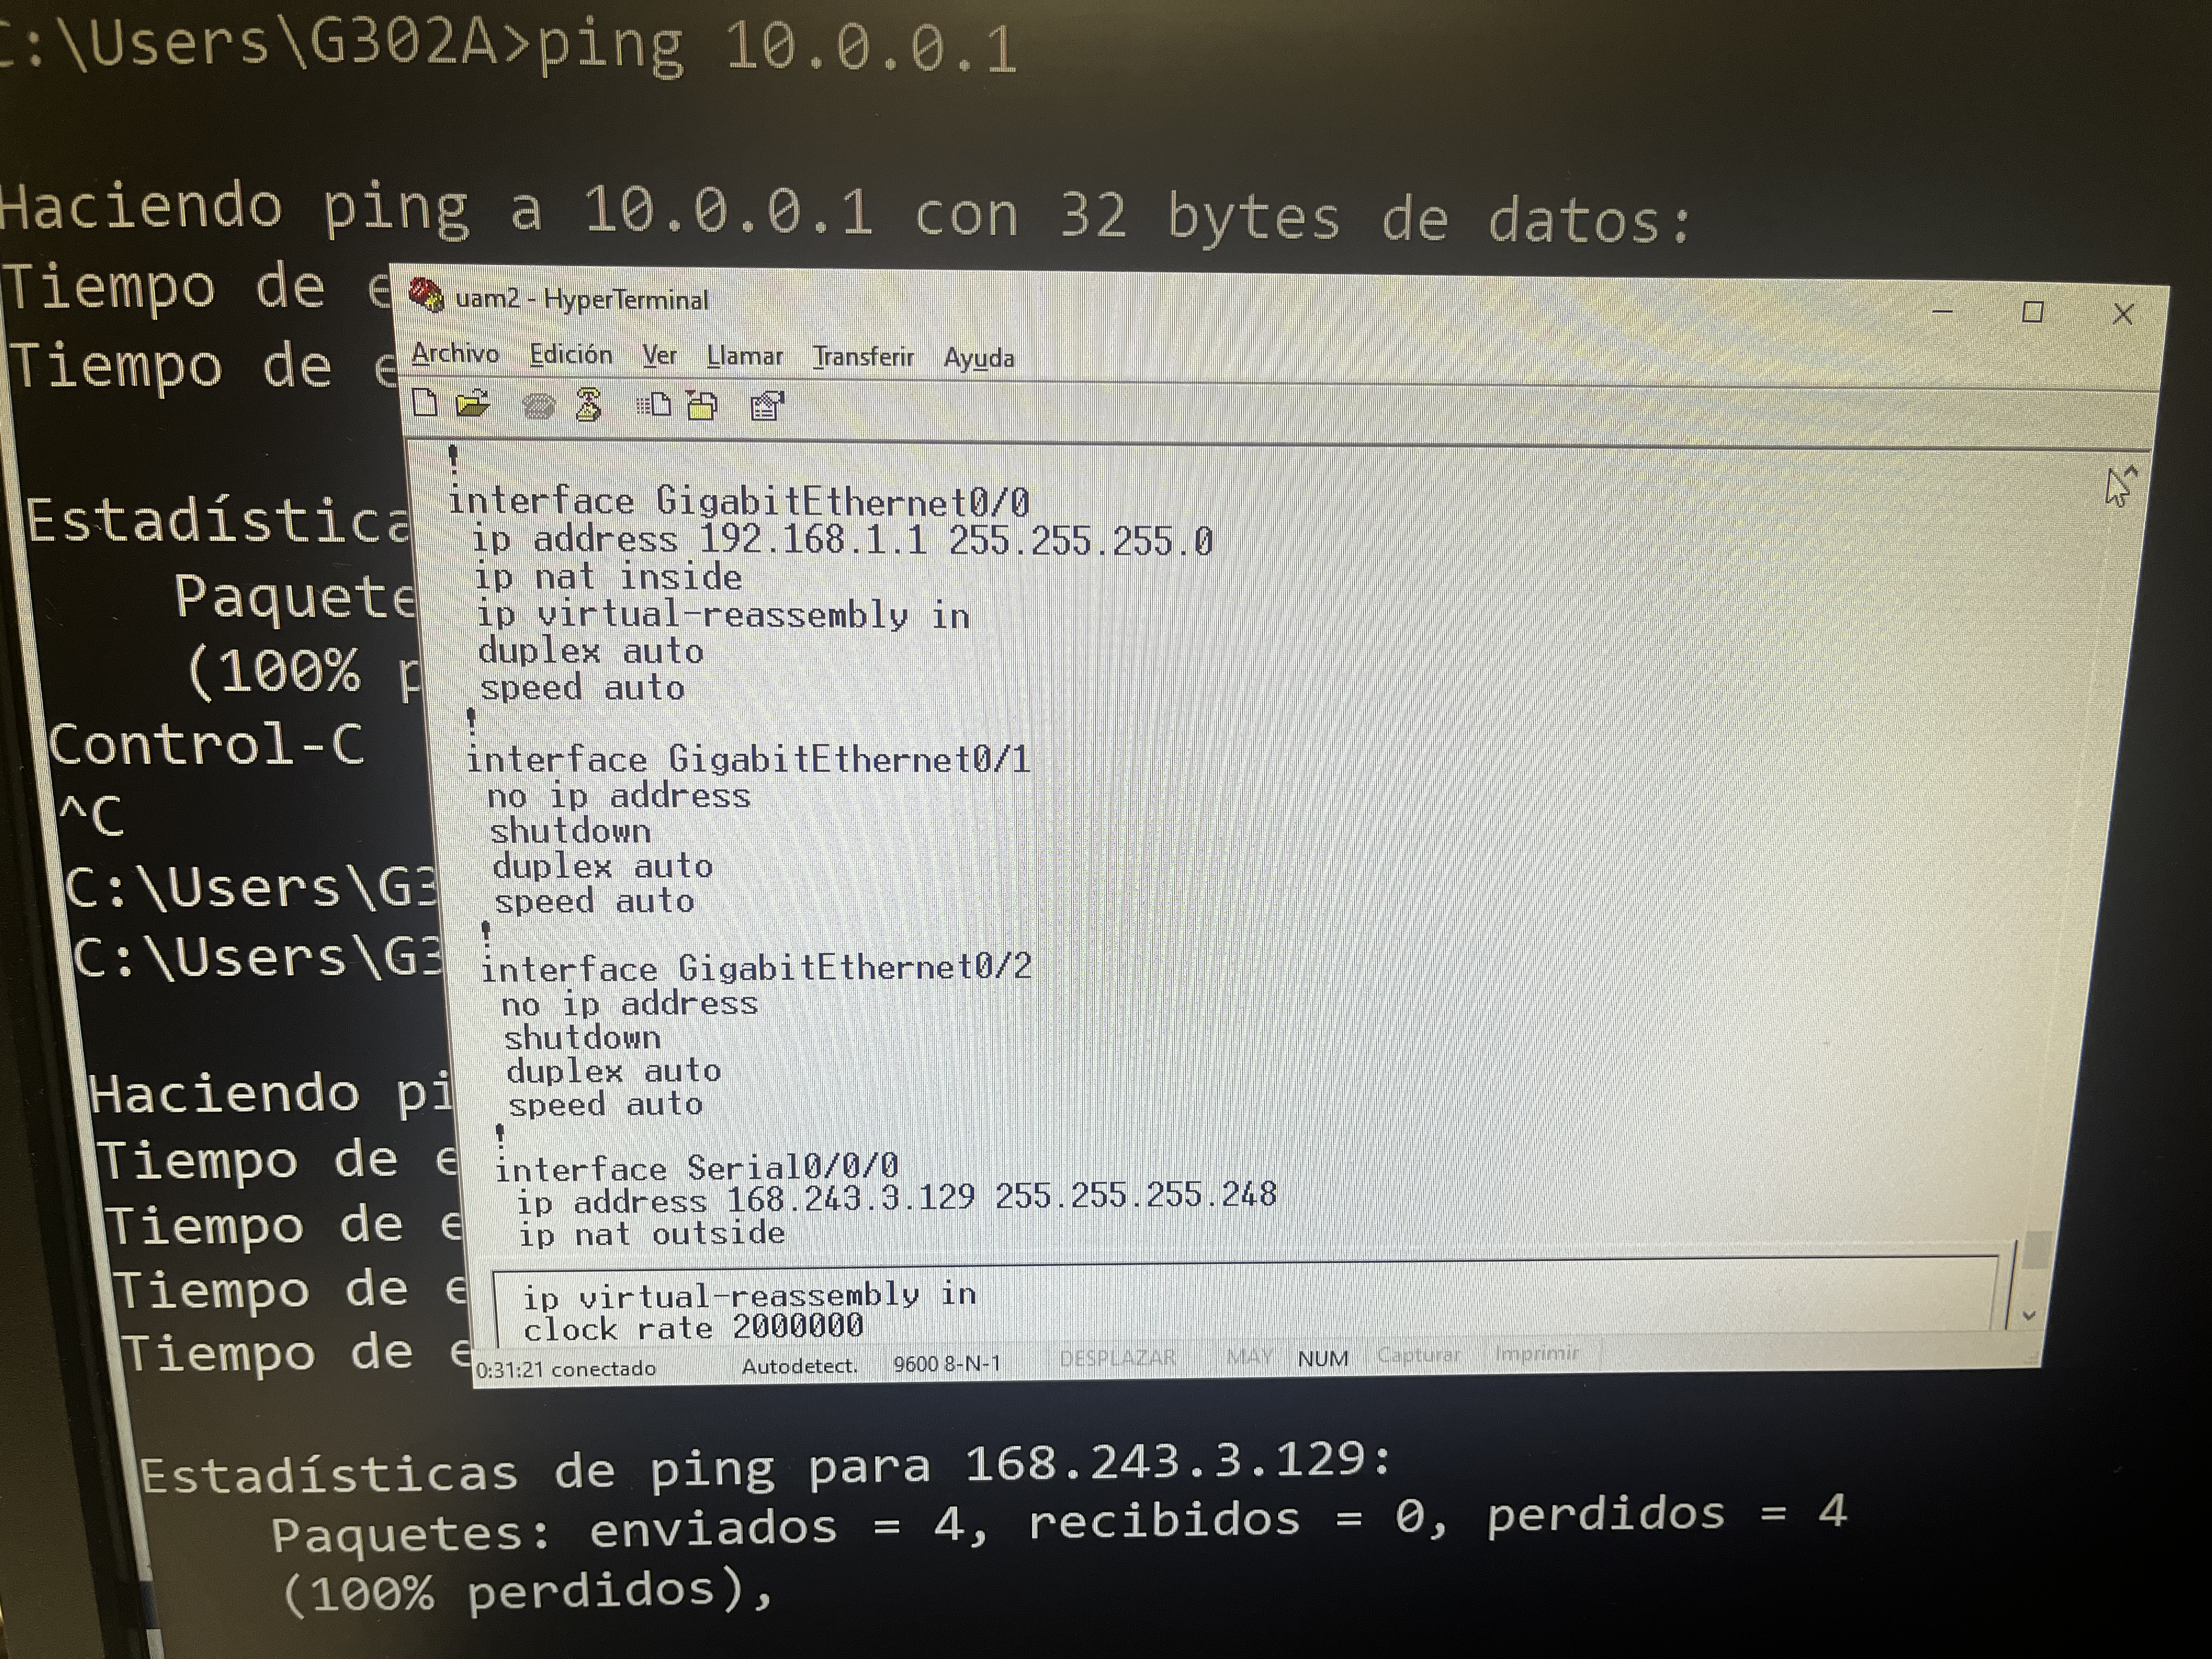
\includegraphics[width=0.8\textwidth]{img/3.jpg}
        \caption{Imagen de Ejemplo}
        \label{fig:Imagen_Ejemplo3}
    \end{figure}

    \begin{figure}[H]
        \centering
        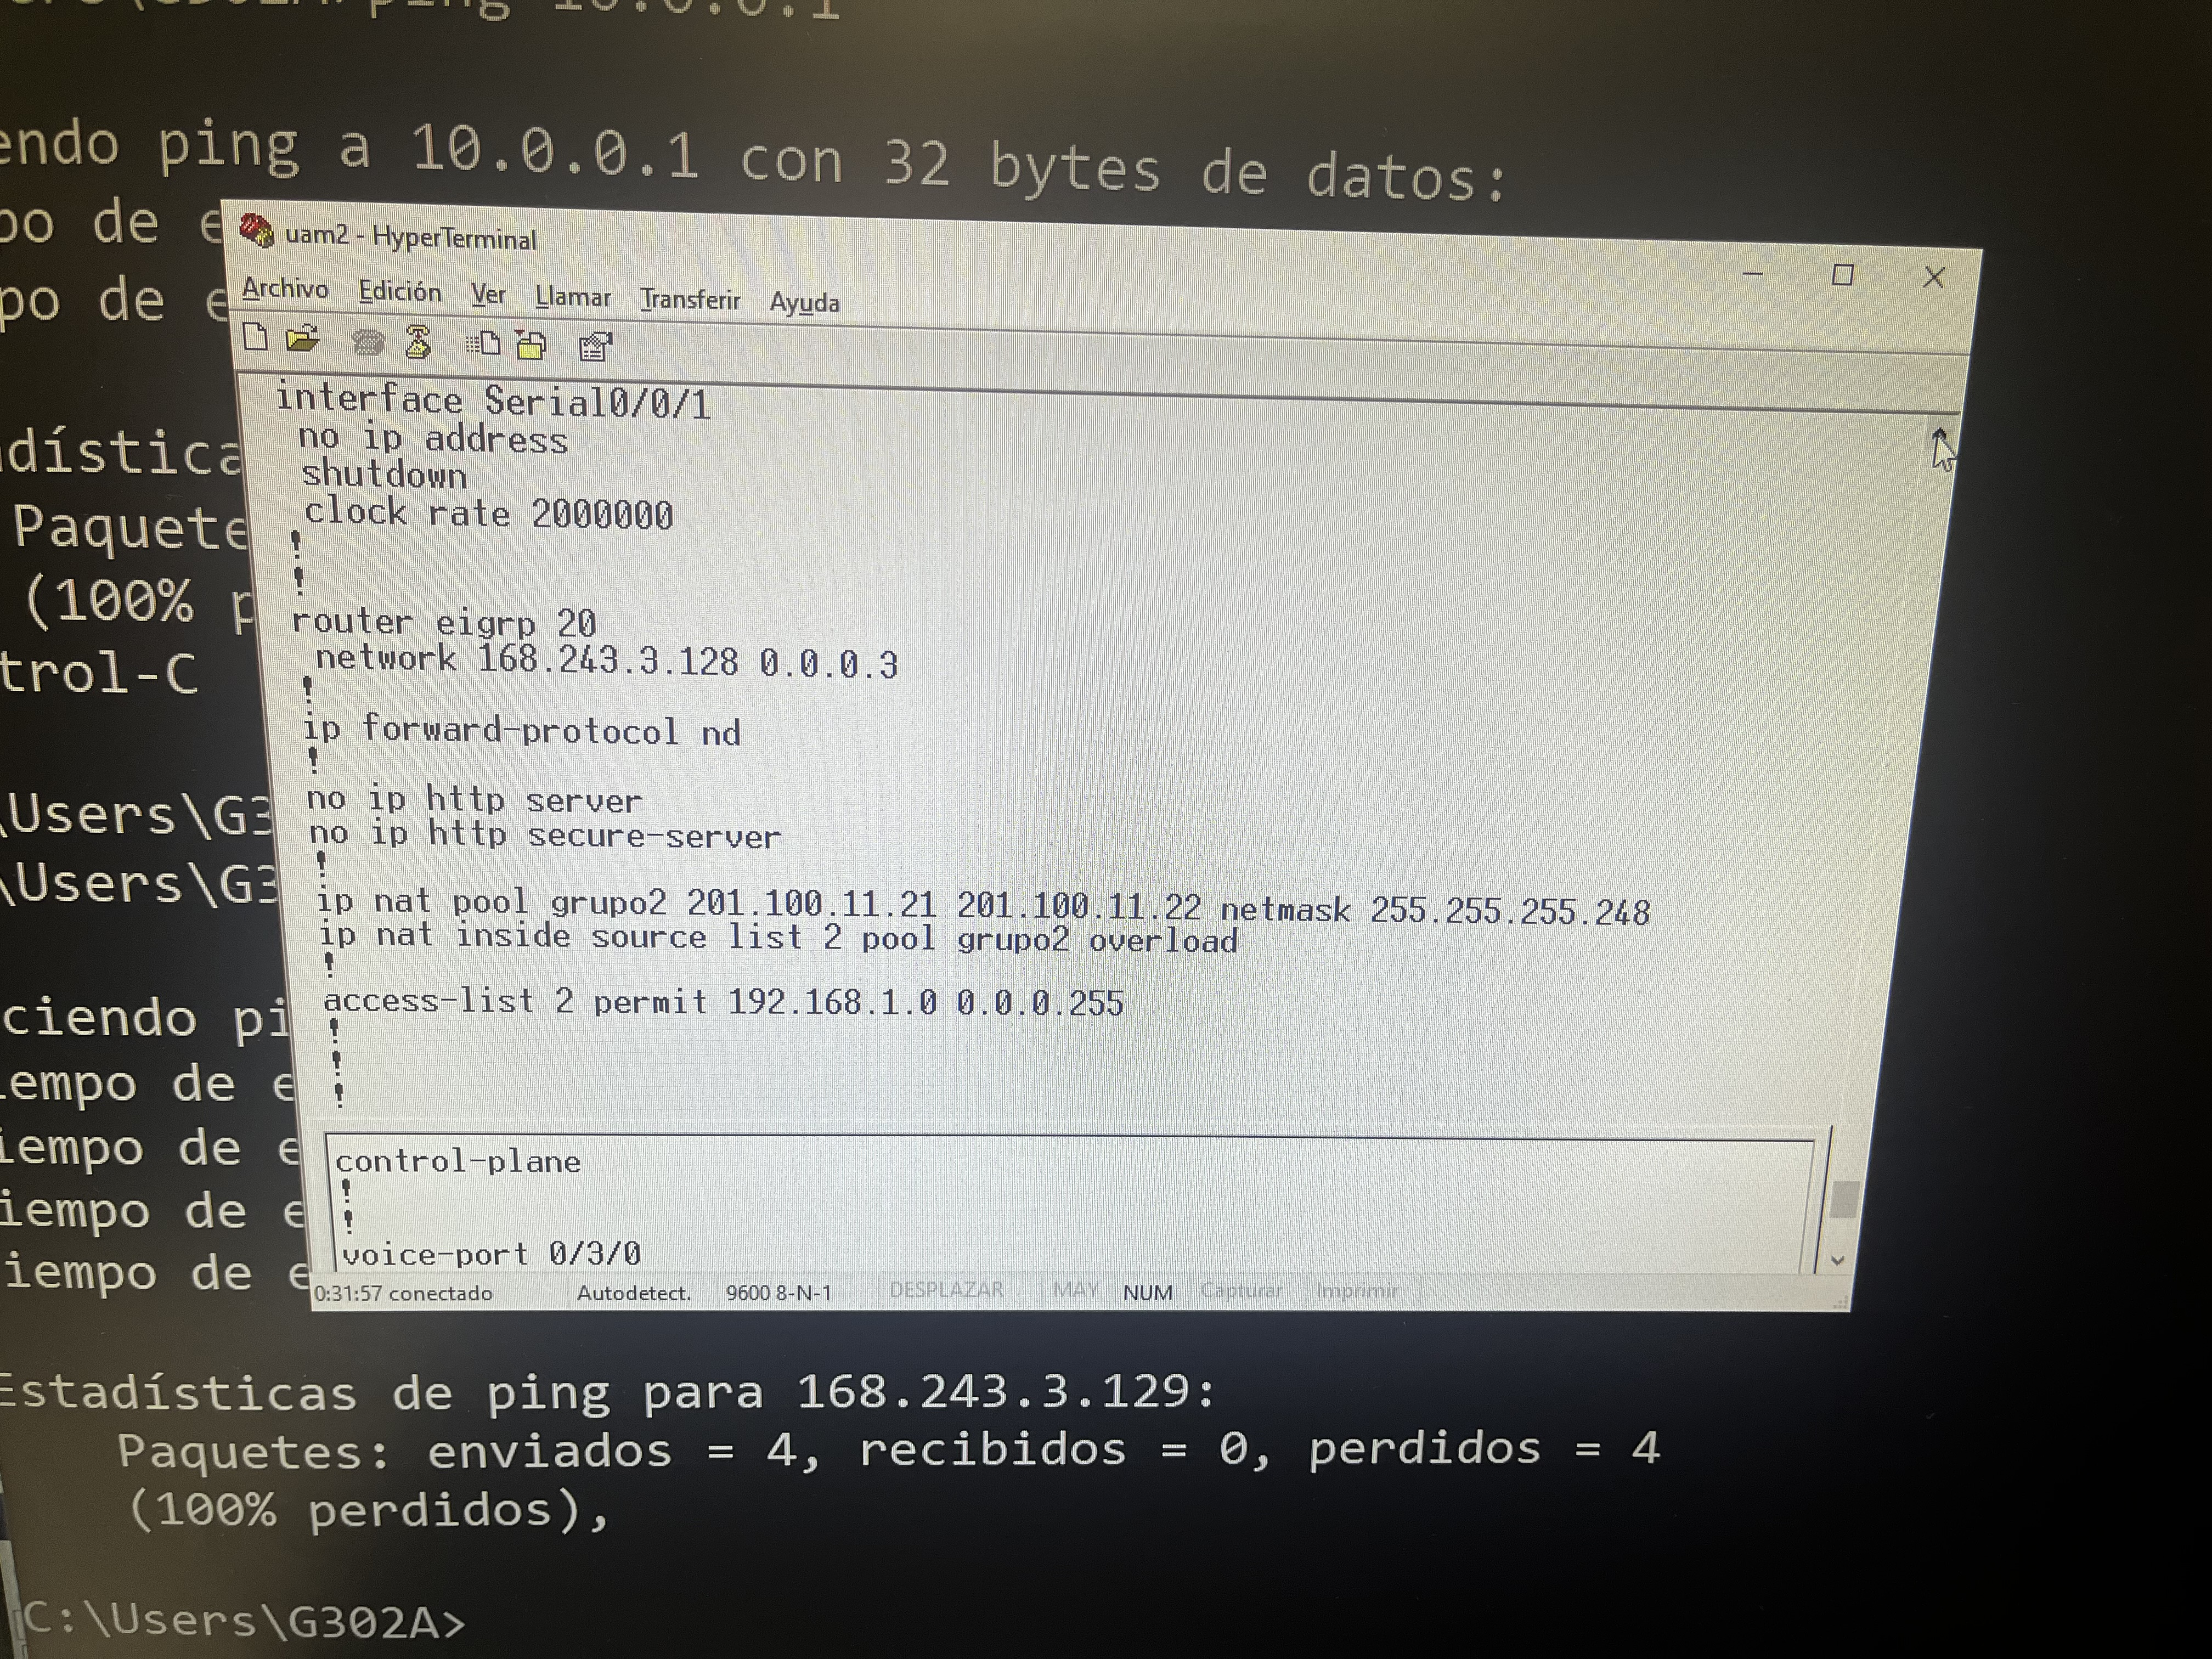
\includegraphics[width=0.8\textwidth]{img/4.jpg}
        \caption{Imagen de Ejemplo}
        \label{fig:Imagen_Ejemplo4}
    \end{figure}

    \begin{figure}[H]
        \centering
        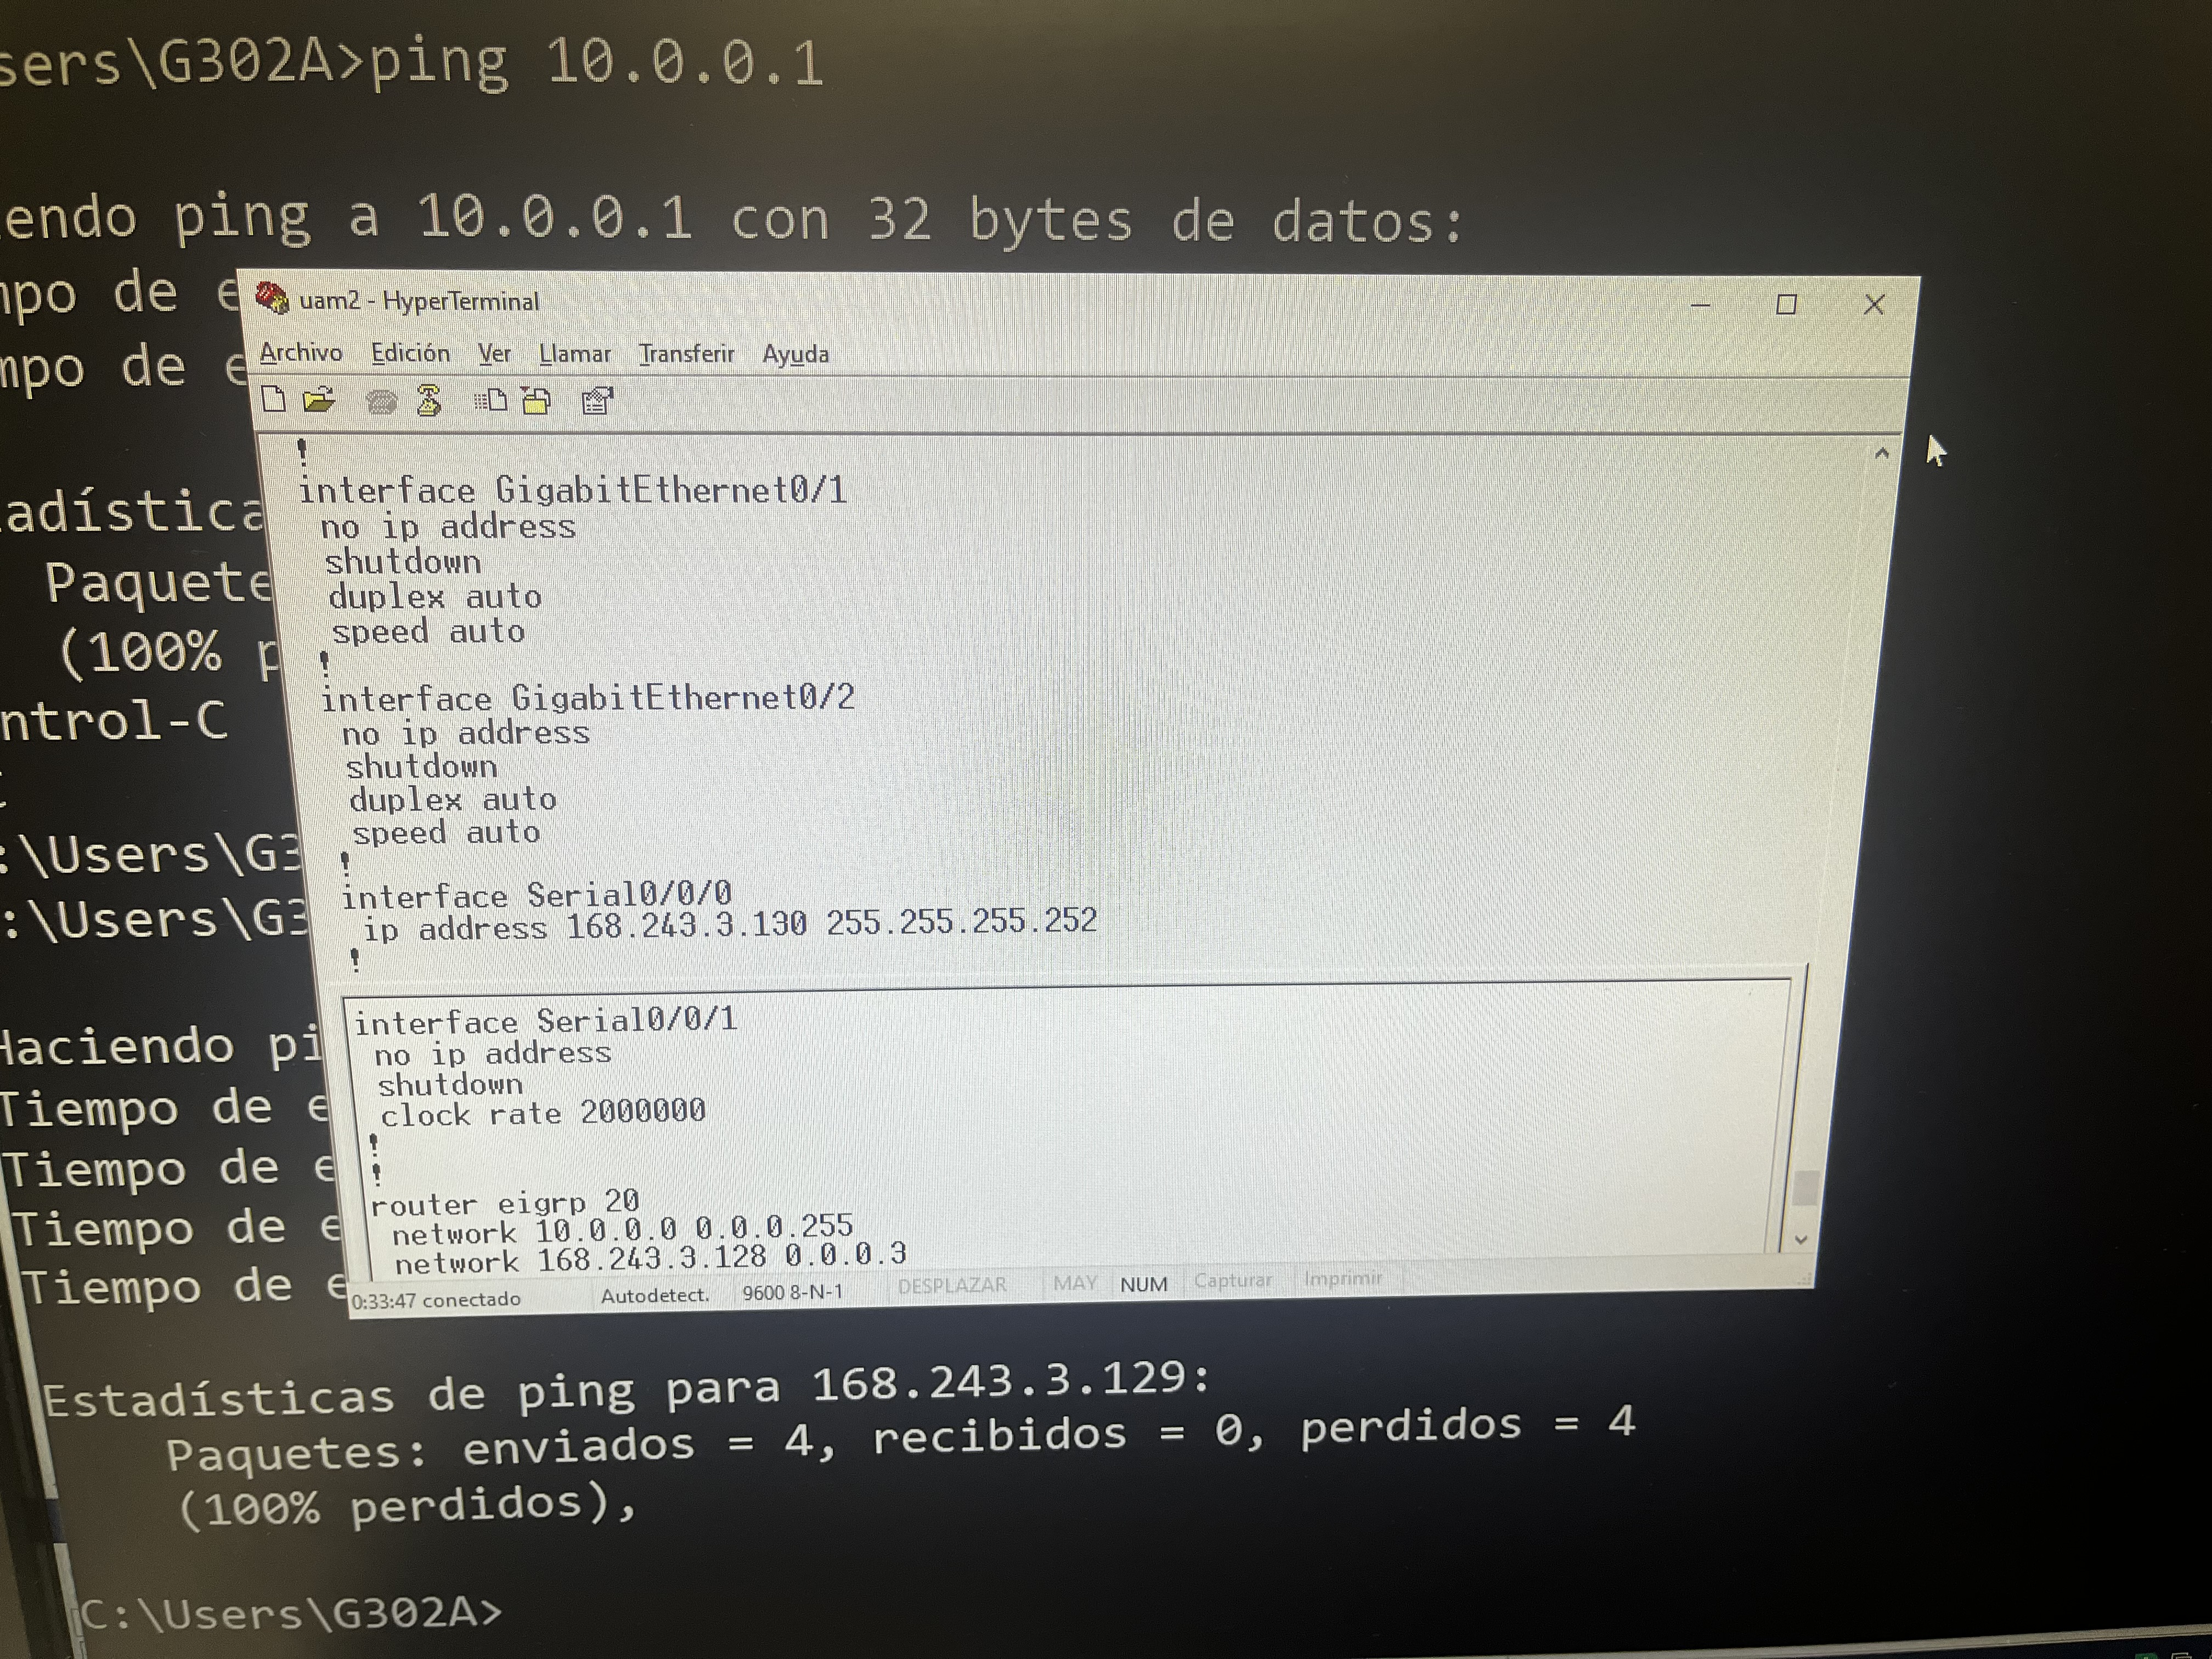
\includegraphics[width=0.8\textwidth]{img/5.jpg}
        \caption{Imagen de Ejemplo}
        \label{fig:Imagen_Ejemplo5}
    \end{figure}

    \begin{figure}[H]
        \centering
        \includegraphics[width=0.8\textwidth]{img/6.jpg}
        \caption{Imagen de Ejemplo}
        \label{fig:Imagen_Ejemplo6}
    \end{figure}



\section{Conclusiones}

% --- Para agregar un apéndice
%\newpage
%\appendix
%\appendixpage
%\addappheadtotoc
%\section{Nombre del apéndice}